\documentclass[tikz,border=12pt]{standalone}
\usepackage{tikz}
\usetikzlibrary{positioning}

\begin{document}
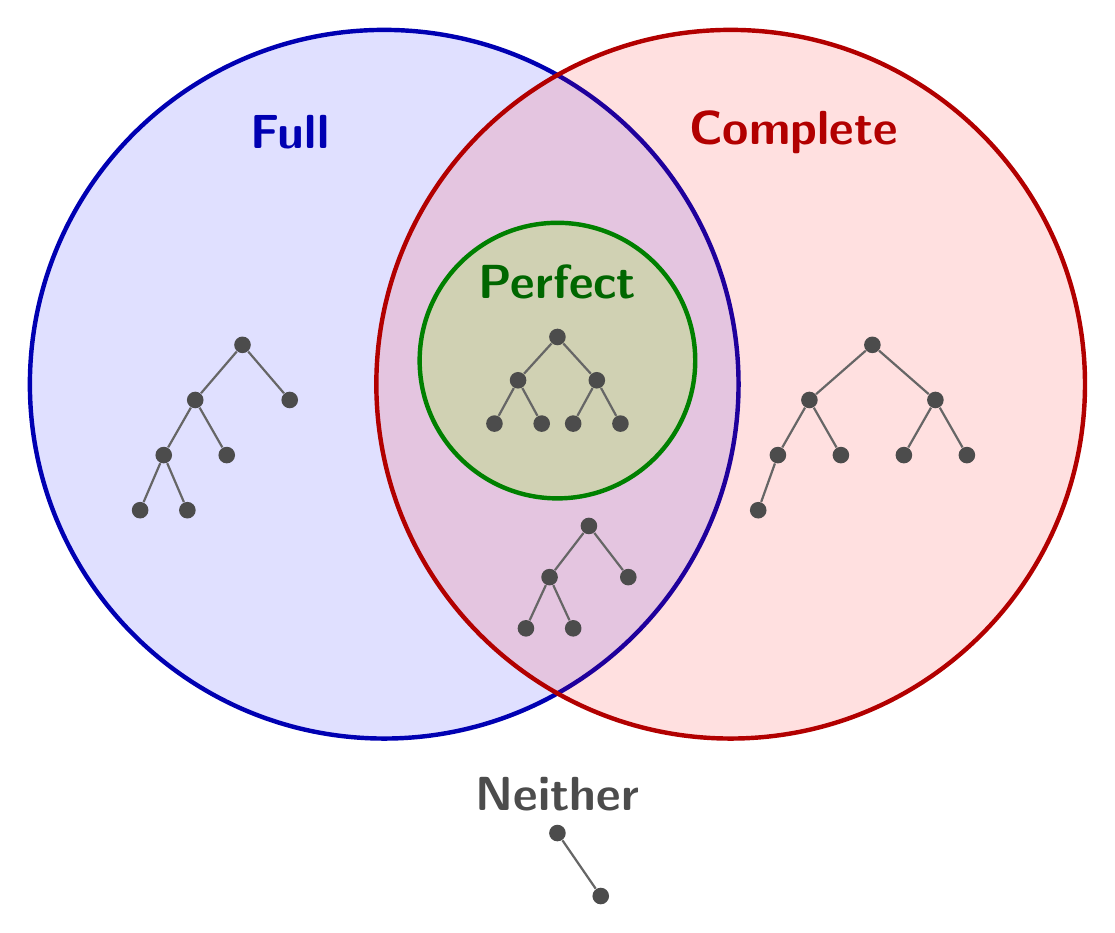
\begin{tikzpicture}[
    every node/.style={font=\sffamily},
    tnode/.style={circle, fill=black!70, inner sep=0pt, minimum size=6pt},
    tedge/.style={thick, black!60},
]

% Draw the two main circles
\node[draw=blue!70!black, fill=blue, circle, minimum size=9cm, fill opacity=0.12, line width=1.6pt] (Full) at (-2.2, 0) {};
\node[draw=red!70!black, fill=red, circle, minimum size=9cm, fill opacity=0.12, line width=1.6pt] (Complete) at (2.2, 0) {};

% Perfect circle inside the intersection
\node[draw=green!50!black, fill=green!50!yellow, circle, minimum size=3.5cm, fill opacity=0.2, line width=1.6pt] (Perfect) at (0, 0.3) {};

% Title labels inside each circle
\node[font=\sffamily\LARGE\bfseries, blue!70!black] at (-3.4, 3.2) {Full};
\node[font=\sffamily\LARGE\bfseries, red!70!black] at (3.0, 3.2) {Complete};
\node[font=\sffamily\LARGE\bfseries, green!40!black] at (0, 1.3) {Perfect};

% ================================================================
% FULL ONLY: 7-node full tree, height 3 (not complete)
%       .
%      / \
%     .   .
%    / \
%   .   .
%  / \
% .   .
% ================================================================
\begin{scope}[shift={(-4.0, 0.5)}]
    \node[tnode] (f1) at (0, 0) {};
    \node[tnode] (f2) at (-0.6, -0.7) {};
    \node[tnode] (f3) at (0.6, -0.7) {};
    \node[tnode] (f4) at (-1.0, -1.4) {};
    \node[tnode] (f5) at (-0.2, -1.4) {};
    \node[tnode] (f6) at (-1.3, -2.1) {};
    \node[tnode] (f7) at (-0.7, -2.1) {};
    \draw[tedge] (f1)--(f2) (f1)--(f3) (f2)--(f4) (f2)--(f5) (f4)--(f6) (f4)--(f7);
\end{scope}

% ================================================================
% COMPLETE ONLY: 8-node complete tree, height 3 (not full)
%         .
%       /   \
%      .     .
%     / \   / \
%    .   . .   .
%   /
%  .
% ================================================================
\begin{scope}[shift={(4.0, 0.5)}]
    \node[tnode] (c1) at (0, 0) {};
    \node[tnode] (c2) at (-0.8, -0.7) {};
    \node[tnode] (c3) at (0.8, -0.7) {};
    \node[tnode] (c4) at (-1.2, -1.4) {};
    \node[tnode] (c5) at (-0.4, -1.4) {};
    \node[tnode] (c6) at (0.4, -1.4) {};
    \node[tnode] (c7) at (1.2, -1.4) {};
    \node[tnode] (c8) at (-1.45, -2.1) {};
    \draw[tedge] (c1)--(c2) (c1)--(c3) (c2)--(c4) (c2)--(c5) (c3)--(c6) (c3)--(c7) (c4)--(c8);
\end{scope}

% ================================================================
% PERFECT: 7-node perfect tree (height 2, 4 leaves)
%       .
%      / \
%     .   .
%    /\ / \
%   . .  . .
% ================================================================
\begin{scope}[shift={(0, 0.05)}]
    \node[tnode] (p1) at (0, 0.55) {};
    \node[tnode] (p2) at (-0.5, 0) {};
    \node[tnode] (p3) at (0.5, 0) {};
    \node[tnode] (p4) at (-0.8, -0.55) {};
    \node[tnode] (p5) at (-0.2, -0.55) {};
    \node[tnode] (p6) at (0.2, -0.55) {};
    \node[tnode] (p7) at (0.8, -0.55) {};
    \draw[tedge] (p1)--(p2) (p1)--(p3) (p2)--(p4) (p2)--(p5) (p3)--(p6) (p3)--(p7);
\end{scope}

% ================================================================
% FULL ∩ COMPLETE, NOT PERFECT: 5-node tree
%     .
%    / \
%   .   .
%  / \
% .   .
% ================================================================
\begin{scope}[shift={(0.4, -1.8)}]
    \node[tnode] (fc1) at (0, 0) {};
    \node[tnode] (fc2) at (-0.5, -0.65) {};
    \node[tnode] (fc3) at (0.5, -0.65) {};
    \node[tnode] (fc4) at (-0.8, -1.3) {};
    \node[tnode] (fc5) at (-0.2, -1.3) {};
    \draw[tedge] (fc1)--(fc2) (fc1)--(fc3) (fc2)--(fc4) (fc2)--(fc5);
\end{scope}

% ================================================================
% NEITHER: root with only a right child
%   .
%    \
%     .
% ================================================================
\node[font=\sffamily\LARGE\bfseries, gray!60!black] at (0, -5.2) {Neither};
\begin{scope}[shift={(0, -5.7)}]
    \node[tnode] (n1) at (0, 0) {};
    \node[tnode] (n2) at (0.55, -0.8) {};
    \draw[tedge] (n1)--(n2);
\end{scope}

\end{tikzpicture}
\end{document}
